%%%%%%%%%%%%%%%%%%%%%%%%%%%%%%%%%%%%%%%%%%%%%%%%%%%%%%%%%%%%%%%%%%%%%%%%%%%%%%%
%  Formalisation and Physlib: A synergy between AI, mathematics and physics
%  Joseph Tooby-Smith -- University of Sussex, 21 October 2026
%
%  Structure follows the talk plan:
%    1  Trust (lead in)          4  Physlib
%    2  What is formalisation?   5  Community and credit
%    3  Monolithic libraries     6  Conclusion
%
%  STYLE.  Palette is the one from ../Sussex2025.html and ../UCL2026.html:
%  teal, copper, slate.  The furniture is print, not web -- square corners,
%  hairline rules, no shadows, no rounded "cards", no pill badges, and no
%  decorative icons.  A block is marked by a rule above it and a letterspaced
%  label, the way a table or a sidebar is marked in a book.  The only icons
%  in the deck are the GitHub glyphs on the repository badges, where they
%  are doing a job.
%
%  Compile with: pdflatex Sussex2026.tex   (run 3x -- the .nav drives the
%  foot rule, and the frames are fragile)
%%%%%%%%%%%%%%%%%%%%%%%%%%%%%%%%%%%%%%%%%%%%%%%%%%%%%%%%%%%%%%%%%%%%%%%%%%%%%%%
\documentclass[aspectratio=169,10pt]{beamer}

\usepackage[T1]{fontenc}
\usepackage[utf8]{inputenc}
\usepackage[sfdefault]{FiraSans}
% Fira Mono for \ttfamily: it matches Fira Sans, and unlike cmtt it has a
% real bold -- T1/cmtt/bx does not exist, so \bfseries on the mono labels
% was silently falling back to regular weight.
\usepackage[scaled=0.88]{FiraMono}
\usefonttheme[onlymath]{serif}
\usepackage{amsmath,amssymb}
\usepackage{microtype}
\usepackage{tikz}
\usepackage{graphicx}
\usepackage{listings}
\usepackage{fontawesome5}
\usepackage[most]{tcolorbox}
\setlength{\fboxrule}{0.6pt}
\setlength{\fboxsep}{0pt}
\usetikzlibrary{calc,positioning,arrows.meta}

\graphicspath{{../Images/}{Images/}}

\hypersetup{
  pdftitle={Physics 2.0: a plan for the future},
  pdfauthor={Joseph Tooby-Smith},
  pdfsubject={Formalisation, Lean, Physlib},
  pdfkeywords={Lean, Physlib, Mathlib, formalisation, AI},
  colorlinks=false, pdfborder={0 0 0},
}

%%%%%%%%%%%%%%%%%%%%%%%%%%%%%%%%%%%%%%%%%%%%%%%%%%%%%%%%%%%%%%%%%%%%%%%%%%%%%%%
%  PALETTE  (from ../Sussex2025.html, ../UCL2026.html, ../IAMP.html)
%%%%%%%%%%%%%%%%%%%%%%%%%%%%%%%%%%%%%%%%%%%%%%%%%%%%%%%%%%%%%%%%%%%%%%%%%%%%%%%
% Two accents and nothing else: a deep teal and its warm complement.  Every
% colour that carries TEXT is at 4.5:1 or better on the page ground, measured,
% not eyeballed -- the old #27AE60 green (2.73:1) and the base teal (2.84:1)
% were both below the 3:1 floor and both were being used for text.
%
%                        on #F9F9F9   on #2F3B4C
%   jttealink  #246B76      5.80         --        text, links, the turnstile
%   jtcopper   #A8432E      5.69         --        text and marks, warm side
%   jtslate    #2F3B4C     10.78         --        body and headings
%   jtgrey     #5A6471      5.71         --        captions and small print
%   jtteal     #4CA1AF       --         3.80       ON DARK only, and the foot bar
\definecolor{jtteal}  {HTML}{4CA1AF}   % light teal: dark grounds, foot bar, tint
\definecolor{jttealink}{HTML}{246B76}  % teal for text on paper
\definecolor{jtcopper}{HTML}{A8432E}   % the warm complement, text-safe
\definecolor{jtslate} {HTML}{2F3B4C}   % headings, dark ground
\definecolor{jtgrey}  {HTML}{5A6471}   % muted text
\definecolor{jtpaper} {HTML}{F9F9F9}   % page ground
\definecolor{jtmist}  {HTML}{C4E0E5}   % pale teal, used only as a tint

% kept as an alias so older call sites still resolve
\definecolor{jtcopperink}{HTML}{A8432E}
\definecolor{jtrule}     {HTML}{D5DBE1}   % hairlines

% The dark ground of the title, dividers and closing, and the colours that sit
% on it.  Lightening the ground costs contrast, so the muted text and the mark
% colour were lightened with it rather than left to fail:
%
%                        on #3E5063
%   jtondark   #F2F5F7      7.57     title and section text
%   jtondarkm  #B8C6D2      4.76     muted text        (was 3.49 on this ground)
%   jtondarka  #6FC0CC      3.98     rules and marks   (was 2.77 on this ground)
%
% jtground is separate from jtslate on purpose: jtslate is the body-text
% colour on light slides and must stay dark.
\definecolor{jtground}  {HTML}{3E5063}
% A second, deeper ground used ONLY by the Physics 1.0 / 2.0 pair, so they do
% not read as another title slide.  Hue-shifted toward the deck's teal, and
% darker, so every on-dark colour gains contrast rather than losing it:
% text 9.75:1, muted 6.12:1, accent 5.13:1 (vs 7.57 / 4.76 / 3.98 on jtground).
\definecolor{jtgroundalt}{HTML}{27424B}
% A pale warm ground that marks the slides which state a PROBLEM.  Distinct
% enough to be read at a glance, quiet enough not to compete with the dark
% title and divider slides.  Slate on it is 10.2:1.
\definecolor{jtproblembg}{HTML}{FBF3F0}
\definecolor{jtondark}  {HTML}{F2F5F7}
\definecolor{jtondarkm} {HTML}{B8C6D2}
\definecolor{jtondarka} {HTML}{6FC0CC}

%%%%%%%%%%%%%%%%%%%%%%%%%%%%%%%%%%%%%%%%%%%%%%%%%%%%%%%%%%%%%%%%%%%%%%%%%%%%%%%
%  BACKGROUNDS
%  A hairline along the foot shows how far through the deck we are.  Before
%  the .nav exists \inserttotalframenumber is 1, so clamp the fraction or a
%  first pass on a clean tree overflows a TeX dimension.
%%%%%%%%%%%%%%%%%%%%%%%%%%%%%%%%%%%%%%%%%%%%%%%%%%%%%%%%%%%%%%%%%%%%%%%%%%%%%%%
\newcommand{\jtFootRule}[1]{%
  \ifnum\inserttotalframenumber>0\relax
    \pgfmathsetmacro{\jtfrac}{min(1,\insertframenumber/\inserttotalframenumber)}%
  \else
    \def\jtfrac{0}%
  \fi
  \fill[#1] (current page.south west)
    rectangle ([xshift=\jtfrac\paperwidth,yshift=0.055cm]current page.south west);}

\newcommand{\jtBackground}{%
  \begin{tikzpicture}[remember picture,overlay]
    \fill[jtpaper] (current page.south west) rectangle (current page.north east);
    \jtFootRule{jtteal}
  \end{tikzpicture}%
}

\newcommand{\jtBackgroundDark}{%
  \begin{tikzpicture}[remember picture,overlay]
    \fill[jtground] (current page.south west) rectangle (current page.north east);
    \jtFootRule{jtondarka}
  \end{tikzpicture}%
}

% The Physics 1.0 / 2.0 ground.
\newcommand{\jtBackgroundAlt}{%
  \begin{tikzpicture}[remember picture,overlay]
    \fill[jtgroundalt] (current page.south west) rectangle (current page.north east);
    \jtFootRule{jtondarka}
  \end{tikzpicture}%
}

% Problem slides: same furniture, warmer paper.
\newcommand{\jtBackgroundProblem}{%
  \begin{tikzpicture}[remember picture,overlay]
    \fill[jtproblembg] (current page.south west) rectangle (current page.north east);
    \jtFootRule{jtcopper}
  \end{tikzpicture}%
}
% Wrap a frame in this to mark it as stating a problem.
\newenvironment{jtproblem}{%
  \begingroup\setbeamertemplate{background}{\jtBackgroundProblem}%
}{\endgroup}


\setbeamertemplate{background}{\jtBackground}

%%%%%%%%%%%%%%%%%%%%%%%%%%%%%%%%%%%%%%%%%%%%%%%%%%%%%%%%%%%%%%%%%%%%%%%%%%%%%%%
%  TYPE
%    \jtlabel{...}  a small bold lowercase label in the accent colour
%    \jtbody        body text inside a block
%    \jtmeta        captions, attributions, small print
%%%%%%%%%%%%%%%%%%%%%%%%%%%%%%%%%%%%%%%%%%%%%%%%%%%%%%%%%%%%%%%%%%%%%%%%%%%%%%%
% Labels are set lowercase in the mono face, the way an identifier is written
% in source.  Deliberately not letterspaced caps: that, over a rule, on a
% rounded card, is the house style of every generated deck.
\newcommand{\jtlabel}[1]{{\bfseries\fontsize{8.5}{10.5}\selectfont
  \MakeLowercase{#1}}}
% A heading-weight label that keeps its capitals, for the few blocks whose
% label is doing real work rather than just naming a slot.
\newcommand{\jtlabelcap}[1]{{\bfseries\fontsize{11.5}{14}\selectfont #1}}
\newcommand{\jtbody}{\small}
\newcommand{\jtmeta}{\footnotesize}

%%%%%%%%%%%%%%%%%%%%%%%%%%%%%%%%%%%%%%%%%%%%%%%%%%%%%%%%%%%%%%%%%%%%%%%%%%%%%%%
%  BEAMER FURNITURE
%%%%%%%%%%%%%%%%%%%%%%%%%%%%%%%%%%%%%%%%%%%%%%%%%%%%%%%%%%%%%%%%%%%%%%%%%%%%%%%
\setbeamertemplate{navigation symbols}{}
\setbeamersize{text margin left=0.9cm,text margin right=0.9cm}
\setbeamercolor{normal text}{fg=jtslate}
\setbeamercolor{frametitle}{fg=jtslate}
\setbeamerfont{frametitle}{size=\Large,series=\bfseries}
\setbeamertemplate{itemize item}{\raisebox{0.2ex}{\tiny\textbullet}}
\setbeamercolor{itemize item}{fg=jttealink}
\setlength{\parskip}{2pt}
\setlength{\leftmargini}{1.2em}
\setlength{\abovedisplayskip}{4pt}
\setlength{\belowdisplayskip}{2pt}
\setlength{\abovedisplayshortskip}{4pt}
\setlength{\belowdisplayshortskip}{2pt}

% The running section name, reset by \jtpart at each divider.  It sits above
% the frame title as a kicker, the way a running head sits on a book page.
\newcommand{\jtkicker}{}
\newcommand{\jtsetkicker}[1]{\gdef\jtkicker{#1}}

% The turnstile, entailment: "from what has been assumed, this follows".  It
% hangs in the left margin beside every frame title and opens every section
% divider.  It is the one ornament in the deck, and it is the subject's own.
\newcommand{\jtturn}{$\vdash$}

\setbeamertemplate{frametitle}{%
  \vspace*{0.20cm}%
  \begin{minipage}{\dimexpr\paperwidth-1.8cm\relax}
    \raggedright
    {\color{jttealink}\jtturn\hspace{5pt}\jtlabel{\jtkicker}\par}
    \vspace{1pt}
    {\usebeamerfont{frametitle}\usebeamercolor[fg]{frametitle}\insertframetitle\par}
    \vspace{3pt}
    {\color{jtslate}\rule{\linewidth}{0.9pt}}
  \end{minipage}\par\vspace{0.10cm}%
}

\setbeamertemplate{footline}{%
  \hbox{%
    \begin{beamercolorbox}[wd=\paperwidth,ht=2.0ex,dp=3.4ex,%
        leftskip=0.9cm,rightskip=0.9cm]{}%
      {\scriptsize\color{jtgrey}Joseph Tooby-Smith\;\textbullet\;University of Bath}%
      \hfill
      {\scriptsize\color{jtgrey}\insertframenumber}%
    \end{beamercolorbox}}%
}

%%%%%%%%%%%%%%%%%%%%%%%%%%%%%%%%%%%%%%%%%%%%%%%%%%%%%%%%%%%%%%%%%%%%%%%%%%%%%%%
%  BLOCKS
%  No rules at all -- not above a block, not beside one.  A block is a quiet
%  panel: white on the off-white page, or a pale tint for a statement that
%  carries weight.  The accent survives in the label, not in an ornament.
%%%%%%%%%%%%%%%%%%%%%%%%%%%%%%%%%%%%%%%%%%%%%%%%%%%%%%%%%%%%%%%%%%%%%%%%%%%%%%%
\tcbset{
  jtbase/.style={
    enhanced, sharp corners, boxrule=0pt, colback=white,
    left=14pt, right=11pt, top=8pt, bottom=8pt,
    halign=flush left, before skip=5pt, after skip=5pt,
  }
}
% [opts] {accent} {label}  -- label may be empty for an unlabelled block
\newtcolorbox{jtblock}[3][]{jtbase,
  #1,
  before upper={\ifx\relax#3\relax\else{\color{#2}\jtlabel{#3}}\par\vspace{6pt}\fi}}
% same, but the label keeps its capitals and is set to stand out
\newtcolorbox{jtblockcap}[3][]{jtbase,
  #1,
  before upper={\ifx\relax#3\relax\else{\color{#2}\jtlabelcap{#3}}\par\vspace{7pt}\fi}}
% Row variant: every block carrying the same group name (#4) is set to the
% natural height of the tallest one, so a row aligns without a hard-coded
% height that the text can outgrow.  Needs two passes to settle.
\newtcolorbox{jtblockh}[4][]{jtbase, equal height group=#4,
  #1,
  before upper={\ifx\relax#3\relax\else{\color{#2}\jtlabel{#3}}\par\vspace{6pt}\fi}}

% A quiet block on a tinted ground, for a single statement.
\newtcolorbox{jtquote}[2][]{enhanced, sharp corners, boxrule=0pt,
  colback=jtmist!28, left=18pt, right=16pt, top=12pt, bottom=12pt,
  before skip=5pt, after skip=5pt, halign=flush left, #1}

% A named thing, set off by a rule down its left edge.  Used where three or
% four things are being named rather than described.
%   #1 accent  #2 the word  #3 gloss (or {})
\newcommand{\jtstack}[3]{%
  {\color{#1}\fontsize{17}{21}\selectfont\bfseries\raggedright #2\par}
  \ifx\relax#3\relax\else\vspace{5pt}{\jtmeta\color{jtgrey}\raggedright #3\par}\fi}

% One quiet panel naming a single thing -- a row of these reads as separate
% items, where bare stacked words read as a block of text.
% Defined here, not in the frame: \newcommand with an argument inside a frame
% body breaks, because beamer re-scans the body.
\newcommand{\jtrole}[1]{%
  \begin{jtblock}[top=7pt,bottom=7pt,before skip=3pt,after skip=3pt]{jttealink}{}
    {\fontsize{14}{18}\selectfont\bfseries\color{jtslate}#1\par}
  \end{jtblock}}

% A figure set large, with its label beneath.  #1 accent  #2 figure  #3 label
\newcommand{\jtfigure}[3]{%
  {\color{#1}\fontsize{34}{36}\selectfont\bfseries #2\par}
  \vspace{6pt}
  {\color{jtslate}\fontsize{13}{17}\selectfont\bfseries #3\par}}

% The Physics 1.0 and Physics 2.0 tables are a matched pair: same ground,
% same header, same row metrics.  They share this machinery so they cannot
% drift apart.  \jtstate is one state, \jtshift is a state changing.
\newcommand{\jtrowhead}[1]{{\color{jttealink}\jtlabel{#1}\par}\vspace{2pt}}
\newcommand{\jtstate}[2]{%
  \jtrowhead{#1}%
  {\fontsize{15}{20}\selectfont{\color{jtslate}#2}\par}
  \vspace{9pt}}

% before -> after, on the dark ground.  #1 tenet, #2 before, #3 after
\newcommand{\jtshift}[3]{%
  \jtrowhead{#1}%
  {\fontsize{15}{20}\selectfont
    {\color{jtgrey}#2}\quad{\color{jtcopper}$\rightarrow$}\quad
    {\color{jtslate}\bfseries #3}\par}
  \vspace{9pt}}

% Numbered points.  The numeral hangs in the accent colour.
\newcommand{\jtnum}[3]{{\fontsize{16}{21}\selectfont
  \hangindent=1.6em \hangafter=1
  \makebox[1.6em][l]{\color{#1}\bfseries#2}{\color{jtslate}#3}\par}}
\newcommand{\jtnumxs}[3]{{\fontsize{12.5}{17}\selectfont
  \hangindent=1.6em \hangafter=1
  \makebox[1.6em][l]{\color{#1}\bfseries#2}{\color{jtslate}#3}\par}}
\newcommand{\jtnumsm}[3]{{\fontsize{14}{19}\selectfont
  \hangindent=1.6em \hangafter=1
  \makebox[1.6em][l]{\color{#1}\bfseries#2}{\color{jtslate}#3}\par}}

%%%%%%%%%%%%%%%%%%%%%%%%%%%%%%%%%%%%%%%%%%%%%%%%%%%%%%%%%%%%%%%%%%%%%%%%%%%%%%%
%  REPOSITORY BADGE
%  Deliberately GitHub-like -- it is quoting a page the audience knows -- so
%  this is the one place in the deck that keeps its icons.
%  #1 owner  #2 repo  #3 url  #4 blurb  #5 stats
%%%%%%%%%%%%%%%%%%%%%%%%%%%%%%%%%%%%%%%%%%%%%%%%%%%%%%%%%%%%%%%%%%%%%%%%%%%%%%%
\newtcolorbox{jtbadge}{enhanced, nobeforeafter, box align=center,
  sharp corners, width=4.4cm, height=4.55cm, valign=top, halign=flush left,
  colback=white, colframe=jtrule, boxrule=0.9pt,
  left=11pt,right=11pt,top=10pt,bottom=10pt}
\newcommand{\jtrepo}[5]{%
  \begin{jtbadge}
    {\color{jtgrey}\fontsize{15}{15}\selectfont\faIcon{github}}\par
    \vspace{7pt}
    % \href takes a box, not a paragraph, so the two lines go in a \parbox.
    \href{#3}{\parbox{\linewidth}{\raggedright
      {\fontsize{6.8}{8}\selectfont\color{jtgrey}#1\,/}\\[1.5pt]
      {\fontsize{14}{16}\selectfont\bfseries\color{jtslate}#2}}}
    \par\vspace{6pt}
    {\fontsize{7.6}{9.6}\selectfont\color{jtgrey}\raggedright #4\par}
    \vfill
    {\color{jtrule}\rule{\linewidth}{0.7pt}}\par\vspace{4pt}
    {\fontsize{6.8}{9}\selectfont\color{jtgrey}#5\par}
  \end{jtbadge}}

%%%%%%%%%%%%%%%%%%%%%%%%%%%%%%%%%%%%%%%%%%%%%%%%%%%%%%%%%%%%%%%%%%%%%%%%%%%%%%%
%  WIDE REPOSITORY CARD
%  The full-width form used in ../CACS2026 and ../BathSeptember26, for when a
%  single repository is the point of the slide.
%  #1 owner #2 repo #3 url #4 blurb #5 stars #6 forks #7 contributors #8 year
%%%%%%%%%%%%%%%%%%%%%%%%%%%%%%%%%%%%%%%%%%%%%%%%%%%%%%%%%%%%%%%%%%%%%%%%%%%%%%%
\newcommand{\jtrepowide}[8]{%
  \begin{tcolorbox}[enhanced, sharp corners, width=0.94\textwidth,
      colback=white, colframe=jtrule, boxrule=0.9pt,
      left=18pt,right=18pt,top=13pt,bottom=13pt]
    \begin{minipage}[c]{0.09\textwidth}
      {\color{jtgrey}\fontsize{26}{26}\selectfont\faIcon{github}}
    \end{minipage}\hfill
    \begin{minipage}[c]{0.72\textwidth}
      \href{#3}{{\Large\bfseries\color{jtslate}#1\,/\,#2}}\\[4pt]
      {\jtbody\color{jtgrey}\raggedright #4\par}
    \end{minipage}\hfill
    \begin{minipage}[c]{0.15\textwidth}
      \raggedleft
      {\color{jtgrey}\jtlabel{public}}\\[3pt]
      {\color{jtgrey}\jtlabel{Lean 4}}
    \end{minipage}

    \vspace{11pt}{\color{jtrule}\rule{\linewidth}{0.8pt}}\vspace{7pt}

    {\jtmeta\color{jtgrey}%
      \faIcon{star}\;\textbf{#5} stars
      \hspace{1.0em}\faIcon{code-branch}\;\textbf{#6} forks
      \hspace{1.0em}\faIcon{users}\;\textbf{#7} contributors
      \hspace{1.0em}\faIcon{clock}\;started #8}
  \end{tcolorbox}}

%%%%%%%%%%%%%%%%%%%%%%%%%%%%%%%%%%%%%%%%%%%%%%%%%%%%%%%%%%%%%%%%%%%%%%%%%%%%%%%
%  SECTION DIVIDERS
%  A contents list on a slate ground, with the section we are entering picked
%  out.  Edit the six names here and the change lands on every divider.
%%%%%%%%%%%%%%%%%%%%%%%%%%%%%%%%%%%%%%%%%%%%%%%%%%%%%%%%%%%%%%%%%%%%%%%%%%%%%%%
\newcommand{\jtsecA}{The problem}
\newcommand{\jtsecB}{Truth}
\newcommand{\jtsecC}{Trust}
\newcommand{\jtsecD}{Community}
\newcommand{\jtsecE}{Recognition}
\newcommand{\jtsecF}{Conclusion}

% #1 = section being entered, #2 = this row's number, #3 = this row's name
\newcommand{\jtrow}[3]{%
  \ifnum#1=#2\relax
    \rlap{\hspace*{-0.85cm}{\color{jtondarka}\rule[0.18ex]{0.5cm}{1.4pt}}}%
    {\color{jtondark}\bfseries #3}%
  \else
    {\color{jtondarkm}#3}%
  \fi\par\vspace{5pt}}

% #1 = section number, #2 = section title
\newcommand{\jtpartbody}[2]{%
  \vfill
  \begin{columns}[T,onlytextwidth]
    \begin{column}{0.56\textwidth}
      {\color{jtondarka}\Large\jtturn}\par
      \vspace{12pt}
      {\color{jtondarkm}\jtlabel{section #1 of 6}\par}
      \vspace{10pt}
      {\color{jtondark}\fontsize{27}{32}\selectfont\bfseries\raggedright #2\par}
    \end{column}
    \begin{column}{0.38\textwidth}
      \vspace{6pt}
      {\jtmeta
        \jtrow{#1}{1}{\jtsecA}%
        \jtrow{#1}{2}{\jtsecB}%
        \jtrow{#1}{3}{\jtsecC}%
        \jtrow{#1}{4}{\jtsecD}%
        \jtrow{#1}{5}{\jtsecE}%
        \jtrow{#1}{6}{\jtsecF}}
    \end{column}
  \end{columns}
  \vfill}

% A divider frame: slate ground, no footline.  #1 number, #2 title, #3 kicker
% for the frames that follow.
\newenvironment{jtsection}[3]{%
  \jtsetkicker{#3}%
  \begingroup
  \setbeamertemplate{background}{\jtBackgroundDark}%
  \setbeamertemplate{footline}{}%
  \begin{frame}[plain]
  \jtpartbody{#1}{#2}%
}{%
  \end{frame}
  \endgroup
}

%%%%%%%%%%%%%%%%%%%%%%%%%%%%%%%%%%%%%%%%%%%%%%%%%%%%%%%%%%%%%%%%%%%%%%%%%%%%%%%
%  LEAN LISTINGS  (ASCII-only source, so pdflatex stays happy)
%%%%%%%%%%%%%%%%%%%%%%%%%%%%%%%%%%%%%%%%%%%%%%%%%%%%%%%%%%%%%%%%%%%%%%%%%%%%%%%
\lstdefinelanguage{lean}{
  morekeywords={theorem,lemma,def,abbrev,example,structure,instance,class,where,
    by,fun,have,show,from,let,match,with,namespace,end,open,variable,
    intro,exact,apply,simp,rfl,ring,unfold,positivity,sorry,Type,Prop,Sort,
    induction,rw,at,
    inductive,cases,Empty,Ne,Nat},
  sensitive=true,
  morecomment=[l]{--},
  morecomment=[s]{/-}{-/},
  morestring=[b]",
}
\lstset{
  language=lean,
  basicstyle=\ttfamily\small\color{jtslate},
  keywordstyle=\bfseries\color{jttealink},
  commentstyle=\itshape\color{jtgrey},
  showstringspaces=false,
  columns=fullflexible,
  breaklines=false,
  aboveskip=1pt, belowskip=1pt,
}

%%%%%%%%%%%%%%%%%%%%%%%%%%%%%%%%%%%%%%%%%%%%%%%%%%%%%%%%%%%%%%%%%%%%%%%%%%%%%%%
\title{Physics 2.0}
\author{Joseph Tooby-Smith}
\date{21 October 2026}

\begin{document}

%%%%%%%%%%%%%%%%%%%%%%%%%%%%%%%%%%%%%%%%%%%%%%%%%%%%%%%%%%%%%%%%%%%%%%%%%%%%%%%
%    TITLE
%%%%%%%%%%%%%%%%%%%%%%%%%%%%%%%%%%%%%%%%%%%%%%%%%%%%%%%%%%%%%%%%%%%%%%%%%%%%%%%
{
\setbeamertemplate{background}{\jtBackgroundDark}
\setbeamertemplate{footline}{}
\begin{frame}[plain]
  \vfill
  \begin{columns}[T,onlytextwidth]
    \begin{column}{0.97\textwidth}
      {\color{jtondarka}\rule{3.2cm}{2pt}}\par
      \vspace{14pt}
      {\color{jtondarkm}\jtlabel{University of Sussex \;\textbullet\; 21 October 2026}\par}
      \vspace{14pt}
      {\color{jtondark}\fontsize{46}{52}\selectfont\bfseries Physics 2.0\par}
      \vspace{10pt}
      {\color{jtondarkm}\fontsize{17}{22}\selectfont
        Formalisation and Physlib: a synergy between AI,
        mathematics and physics\par}
      \vspace{16pt}
      {\color{jtondarkm}\rule{\linewidth}{0.5pt}}\par
      \vspace{12pt}
      {\color{jtondark}\fontsize{13}{16}\selectfont\bfseries Joseph Tooby-Smith\par}
      \vspace{4pt}
      {\color{jtondarkm}\jtmeta University of Bath\par}
      \vspace{14pt}
      {\color{jtondarkm}\jtmeta
        \href{https://github.com/leanprover-community/physlib}{%
          \color{jtondarkm}github.com/leanprover-community/physlib}
        \qquad
        \href{https://josephtoobysmith.com/}{%
          \color{jtondarkm}josephtoobysmith.com}\par}
    \end{column}
  \end{columns}
  \vfill
\end{frame}
}

%%%%%%%%%%%%%%%%%%%%%%%%%%%%%%%%%%%%%%%%%%%%%%%%%%%%%%%%%%%%%%%%%%%%%%%%%%%%%%%
%%  SECTION 1  --  THE PROBLEM
%%%%%%%%%%%%%%%%%%%%%%%%%%%%%%%%%%%%%%%%%%%%%%%%%%%%%%%%%%%%%%%%%%%%%%%%%%%%%%%
\begin{jtsection}{1}{The problem we face}{The problem}
\end{jtsection}

%%%%%%%%%%%%%%%%%%%%%%%%%%%%%%%%%%%%%%%%%%%%%%%%%%%%%%%%%%%%%%%%%%%%%%%%%%%%%%%
%  1.1  THE PROBLEM WE FACE
%%%%%%%%%%%%%%%%%%%%%%%%%%%%%%%%%%%%%%%%%%%%%%%%%%%%%%%%%%%%%%%%%%%%%%%%%%%%%%%
\begin{jtproblem}
\begin{frame}{The problem we face}
  \vfill
  \begin{minipage}{0.94\textwidth}
    \raggedright
    \jtnumsm{jtcopper}{1}{AI is getting better and better.}
    \vspace{11pt}
    \jtnumsm{jtcopper}{2}{We don't know how far it will get.}
    \vspace{11pt}
    \jtnumsm{jtcopper}{3}{The arXiv and journals are being overwhelmed.}
    \vspace{11pt}
    \jtnumsm{jtcopper}{4}{It is hard to know what to trust and what not to.}
  \end{minipage}
  \vfill
\end{frame}
\end{jtproblem}

%%%%%%%%%%%%%%%%%%%%%%%%%%%%%%%%%%%%%%%%%%%%%%%%%%%%%%%%%%%%%%%%%%%%%%%%%%%%%%%
%  1.2  EVIDENCE THAT AI IS GETTING BETTER
%%%%%%%%%%%%%%%%%%%%%%%%%%%%%%%%%%%%%%%%%%%%%%%%%%%%%%%%%%%%%%%%%%%%%%%%%%%%%%%
\begin{frame}{Evidence that AI is getting better}
  \vfill
  \begin{columns}[T,onlytextwidth]

    \begin{column}{0.475\textwidth}
      \begin{jtblockh}[top=6pt,bottom=6pt]{jtcopper}{July 2026}{news}
        {\fontsize{14}{18}\selectfont\bfseries\color{jtslate}
          The Jacobian conjecture\par}
        \vspace{4pt}
        {\jtbody\color{jtslate}Keller, 1939. Counterexample in $\mathbb{C}^{3}$.\par}
        \vfill
        {\jtmeta\color{jtgrey}Alpoge, with Claude Fable 5\par}
      \end{jtblockh}
    \end{column}

    \begin{column}{0.475\textwidth}
      \begin{jtblockh}[top=6pt,bottom=6pt]{jtcopper}{August 2026}{news}
        {\fontsize{14}{18}\selectfont\bfseries\color{jtslate}
          Ten open problems\par}
        \vspace{4pt}
        {\jtbody\color{jtslate}From maths and CS\par}
        \vfill
        {\jtmeta\color{jtgrey}OpenAI ``Astra''\par}
      \end{jtblockh}
    \end{column}

  \end{columns}
  \vspace{2pt}
  \begin{columns}[T,onlytextwidth]

    \begin{column}{0.475\textwidth}
      \begin{jtblockh}[top=6pt,bottom=6pt]{jtcopper}{September 2026}{news}
        {\fontsize{14}{18}\selectfont\bfseries\color{jtslate}
          Navier--Stokes problem\par}
        \vspace{4pt}
        {\jtbody\color{jtslate}Finite time blow-up.\par}
        \vfill
        {\jtmeta\color{jtgrey}AI models\par}
      \end{jtblockh}
    \end{column}

    \begin{column}{0.475\textwidth}
      \begin{jtblockh}[top=6pt,bottom=6pt]{jtcopper}{October 2026}{news}
        {\fontsize{14}{18}\selectfont\bfseries\color{jtslate}
          372 problems\par}
        \vfill
        {\jtmeta\color{jtgrey}OpenAI, internal model\par}
      \end{jtblockh}
    \end{column}

  \end{columns}
  \vfill
\end{frame}

%%%%%%%%%%%%%%%%%%%%%%%%%%%%%%%%%%%%%%%%%%%%%%%%%%%%%%%%%%%%%%%%%%%%%%%%%%%%%%%
%  1.3  PHYSICS 1.0 NO LONGER WORKS
%%%%%%%%%%%%%%%%%%%%%%%%%%%%%%%%%%%%%%%%%%%%%%%%%%%%%%%%%%%%%%%%%%%%%%%%%%%%%%%
\begin{frame}{The conclusion of this}
  \vfill
  \begin{minipage}{0.94\textwidth}
    \raggedright
    {\color{jtslate}\fontsize{22}{30}\selectfont\bfseries
      Physics 1.0 no longer works.\par}
  \end{minipage}
  \vfill
\end{frame}

%%%%%%%%%%%%%%%%%%%%%%%%%%%%%%%%%%%%%%%%%%%%%%%%%%%%%%%%%%%%%%%%%%%%%%%%%%%%%%%
%  1.4  WHAT I THINK
%%%%%%%%%%%%%%%%%%%%%%%%%%%%%%%%%%%%%%%%%%%%%%%%%%%%%%%%%%%%%%%%%%%%%%%%%%%%%%%
\begin{frame}{What I think}
  \vfill
  % epigraph: Popper, The Lesson of This Century (1997)
  {\fontsize{15}{21}\selectfont\itshape\color{jtslate}%
    ``Optimism is a duty. The future is open.''\par}
  \vspace{2pt}
  {\jtmeta\color{jtgrey}--- Karl Popper\par}
  \vspace{18pt}
  \begin{minipage}{0.94\textwidth}
    \raggedright
    \onslide<1->{%
    \jtnumsm{jttealink}{1}{We should optimistically push towards a solution.}}
    \vspace{14pt}
    \onslide<2->{%
    \jtnumsm{jttealink}{2}{Here I will present my solution, an idea I call
      {\bfseries Physics 2.0}.}}
    \vspace{14pt}
    \onslide<3->{%
    \jtnumsm{jttealink}{3}{When doing so, we should bear in mind what AI now
      makes {\bfseries possible}.}}
  \end{minipage}
  \vfill
\end{frame}

%%%%%%%%%%%%%%%%%%%%%%%%%%%%%%%%%%%%%%%%%%%%%%%%%%%%%%%%%%%%%%%%%%%%%%%%%%%%%%%
%  1.5  THINGS TO PRESERVE: FOUR TENETS OF ACADEMIA
%%%%%%%%%%%%%%%%%%%%%%%%%%%%%%%%%%%%%%%%%%%%%%%%%%%%%%%%%%%%%%%%%%%%%%%%%%%%%%%
\begin{frame}{Things to preserve: four tenets of academia}
  \vfill
  \begin{minipage}{0.94\textwidth}
    \raggedright
    {\color{jtslate}\fontsize{26}{36}\selectfont\bfseries
      Truth\par Trust\par Community\par Recognition\par}
  \end{minipage}
  \vfill
\end{frame}

%%%%%%%%%%%%%%%%%%%%%%%%%%%%%%%%%%%%%%%%%%%%%%%%%%%%%%%%%%%%%%%%%%%%%%%%%%%%%%%
%  1.6  PHYSICS 1.0
%%%%%%%%%%%%%%%%%%%%%%%%%%%%%%%%%%%%%%%%%%%%%%%%%%%%%%%%%%%%%%%%%%%%%%%%%%%%%%%
\begin{frame}{Physics 1.0}
  \vfill
  \begin{minipage}{0.96\textwidth}
    \raggedright
  \jtstate{Truth}{Disseminated in academic papers.}
  \jtstate{Trust}{Peer review.}
  \jtstate{Community}{Spends its time writing papers, and reviewing them.}
  \jtstate{Recognition}{Citation counts, and numbers of papers.}
  \end{minipage}
  \vfill
\end{frame}

%%%%%%%%%%%%%%%%%%%%%%%%%%%%%%%%%%%%%%%%%%%%%%%%%%%%%%%%%%%%%%%%%%%%%%%%%%%%%%%
%%  SECTION 2  --  REORGANISING TRUTH
%%%%%%%%%%%%%%%%%%%%%%%%%%%%%%%%%%%%%%%%%%%%%%%%%%%%%%%%%%%%%%%%%%%%%%%%%%%%%%%
\begin{jtsection}{2}{Reorganising truth}{Truth}
\end{jtsection}

%%%%%%%%%%%%%%%%%%%%%%%%%%%%%%%%%%%%%%%%%%%%%%%%%%%%%%%%%%%%%%%%%%%%%%%%%%%%%%%
%  2.1  WHAT IS WRONG WITH PAPERS
%%%%%%%%%%%%%%%%%%%%%%%%%%%%%%%%%%%%%%%%%%%%%%%%%%%%%%%%%%%%%%%%%%%%%%%%%%%%%%%
\begin{jtproblem}
\begin{frame}{What is wrong with papers?}
  \vfill
  \begin{minipage}{0.94\textwidth}
    \raggedright
    \jtnum{jtcopper}{1}{Hard to find information.}
    \vspace{13pt}
    \jtnum{jtcopper}{2}{Hard to reuse.}
    \vspace{13pt}
    \jtnum{jtcopper}{3}{Hard to find connections.}
    \vspace{13pt}
    \jtnum{jtcopper}{4}{Papers are outdated. It is time to find something new.}
  \end{minipage}
  \vfill
\end{frame}
\end{jtproblem}

%%%%%%%%%%%%%%%%%%%%%%%%%%%%%%%%%%%%%%%%%%%%%%%%%%%%%%%%%%%%%%%%%%%%%%%%%%%%%%%
%  2.2  THE SOLUTION
%%%%%%%%%%%%%%%%%%%%%%%%%%%%%%%%%%%%%%%%%%%%%%%%%%%%%%%%%%%%%%%%%%%%%%%%%%%%%%%
\begin{frame}{The solution}
  \vfill
  \begin{jtquote}[top=12pt,bottom=12pt]{jttealink}
    {\fontsize{16}{22}\selectfont\color{jtslate}%
      Store information not in papers, but in an {\bfseries open-source,
      community-run} corpus of knowledge.\par}
  \end{jtquote}

  \vspace{10pt}
  % one box per "hard to" complaint on the previous slide, in the same order
  \begin{columns}[T,onlytextwidth]
    \begin{column}{0.315\textwidth}
      \begin{jtblockh}[top=8pt,bottom=8pt,left=10pt,right=6pt]{jttealink}{}{sol}
        {\jtbody\color{jtslate}Easy to {\bfseries find} information.\par}
      \end{jtblockh}
    \end{column}
    \begin{column}{0.315\textwidth}
      \begin{jtblockh}[top=8pt,bottom=8pt,left=10pt,right=6pt]{jttealink}{}{sol}
        {\jtbody\color{jtslate}Easy to {\bfseries reuse}.\par}
      \end{jtblockh}
    \end{column}
    \begin{column}{0.315\textwidth}
      \begin{jtblockh}[top=8pt,bottom=8pt,left=10pt,right=6pt]{jttealink}{}{sol}
        {\jtbody\color{jtslate}Easy to find {\bfseries connections}.\par}
      \end{jtblockh}
    \end{column}
  \end{columns}

  \vspace{10pt}
  {\jtmeta\color{jtgrey}Similar reason to why {\bfseries SciPy} exists in
    Python.\par}
  \vfill
\end{frame}

%%%%%%%%%%%%%%%%%%%%%%%%%%%%%%%%%%%%%%%%%%%%%%%%%%%%%%%%%%%%%%%%%%%%%%%%%%%%%%%
%  2.3  DISSENT
%%%%%%%%%%%%%%%%%%%%%%%%%%%%%%%%%%%%%%%%%%%%%%%%%%%%%%%%%%%%%%%%%%%%%%%%%%%%%%%
\begin{frame}{Dissent against our solution}
  \vfill
  \begin{minipage}{0.94\textwidth}
    \raggedright
    \jtnum{jtcopper}{1}{Such a corpus of knowledge is hard to maintain.}
    \vspace{13pt}
    \jtnum{jtcopper}{2}{It is hard to keep up to date.}
  \end{minipage}

  \vspace{20pt}
  \begin{jtquote}[top=11pt,bottom=11pt]{jttealink}
    {\fontsize{17}{23}\selectfont\color{jtslate}%
      AI helps with {\bfseries all of this}.\par}
  \end{jtquote}
  \vfill
\end{frame}

%%%%%%%%%%%%%%%%%%%%%%%%%%%%%%%%%%%%%%%%%%%%%%%%%%%%%%%%%%%%%%%%%%%%%%%%%%%%%%%
%  2.4  INGREDIENT 1 OF PHYSICS 2.0  (the badge)
%%%%%%%%%%%%%%%%%%%%%%%%%%%%%%%%%%%%%%%%%%%%%%%%%%%%%%%%%%%%%%%%%%%%%%%%%%%%%%%
\begin{frame}{Ingredient 1 of Physics 2.0}
  \vfill
  \begin{center}
    \jtrepowide{leanprover-community}{Physlib}
      {https://github.com/leanprover-community/physlib}
      {A community-driven project to digitalise results from physics into Lean.}
      {786}{205}{114}{2024}
  \end{center}

  \vspace{14pt}
  {\centering\jtmeta\color{jtgrey}%
    I will explain the details later.\par}
  \vfill
\end{frame}

%%%%%%%%%%%%%%%%%%%%%%%%%%%%%%%%%%%%%%%%%%%%%%%%%%%%%%%%%%%%%%%%%%%%%%%%%%%%%%%
%%  SECTION 3  --  ADJUSTING TRUST
%%%%%%%%%%%%%%%%%%%%%%%%%%%%%%%%%%%%%%%%%%%%%%%%%%%%%%%%%%%%%%%%%%%%%%%%%%%%%%%
\begin{jtsection}{3}{Adjusting trust}{Trust}
\end{jtsection}

%%%%%%%%%%%%%%%%%%%%%%%%%%%%%%%%%%%%%%%%%%%%%%%%%%%%%%%%%%%%%%%%%%%%%%%%%%%%%%%
%  3.1  WHAT IS WRONG WITH PEER REVIEW
%%%%%%%%%%%%%%%%%%%%%%%%%%%%%%%%%%%%%%%%%%%%%%%%%%%%%%%%%%%%%%%%%%%%%%%%%%%%%%%
\begin{jtproblem}
\begin{frame}{What is wrong with peer review?}
  \vfill
  \begin{minipage}{0.94\textwidth}
    \raggedright
    \jtnum{jtcopper}{1}{It does not scale efficiently with AI.}
    \vspace{13pt}
    \jtnum{jtcopper}{2}{Mistakes get into papers, and slip past reviewers.}
  \end{minipage}
  \vfill
\end{frame}
\end{jtproblem}

%%%%%%%%%%%%%%%%%%%%%%%%%%%%%%%%%%%%%%%%%%%%%%%%%%%%%%%%%%%%%%%%%%%%%%%%%%%%%%%
%  3.2  THE MATHEMATICIANS HAVE A SOLUTION
%%%%%%%%%%%%%%%%%%%%%%%%%%%%%%%%%%%%%%%%%%%%%%%%%%%%%%%%%%%%%%%%%%%%%%%%%%%%%%%
\begin{frame}{The mathematicians have a solution}
  \vfill
  \begin{jtquote}[top=14pt,bottom=14pt]{jttealink}
    {\fontsize{21}{28}\selectfont\color{jtslate}%
      It is called {\bfseries formalisation}.\par}
  \end{jtquote}
  \vfill
\end{frame}

%%%%%%%%%%%%%%%%%%%%%%%%%%%%%%%%%%%%%%%%%%%%%%%%%%%%%%%%%%%%%%%%%%%%%%%%%%%%%%%
%  3.3  TECHNICAL INTERLUDE  (opens the formalisation tutorial)
%%%%%%%%%%%%%%%%%%%%%%%%%%%%%%%%%%%%%%%%%%%%%%%%%%%%%%%%%%%%%%%%%%%%%%%%%%%%%%%
{
\setbeamertemplate{background}{\jtBackgroundDark}
\setbeamertemplate{footline}{}
\begin{frame}[plain]
  \vfill
  {\color{jtondarka}\Large\jtturn}\par
  \vspace{14pt}
  {\color{jtondark}\fontsize{30}{36}\selectfont\bfseries Technical interlude\par}
  \vfill
\end{frame}
}

%%%%%%%%%%%%%%%%%%%%%%%%%%%%%%%%%%%%%%%%%%%%%%%%%%%%%%%%%%%%%%%%%%%%%%%%%%%%%%%
%  3.4  WHAT IS AN INTERACTIVE THEOREM PROVER?
%%%%%%%%%%%%%%%%%%%%%%%%%%%%%%%%%%%%%%%%%%%%%%%%%%%%%%%%%%%%%%%%%%%%%%%%%%%%%%%
\begin{frame}{What is an interactive theorem prover?}
  \vfill
  \begin{jtquote}[left=20pt,right=20pt,top=16pt,bottom=16pt]{jttealink}
    {\fontsize{17}{24}\selectfont\color{jtslate}%
      A programming language in which you can write mathematical theorems
      proofs, and definitions, with mathematical
      {\bfseries correctness} and {\bfseries consistency} guaranteed.
      And the definitions you write are {\bfseries executable}.\par}
  \end{jtquote}
  \vfill
\end{frame}

%%%%%%%%%%%%%%%%%%%%%%%%%%%%%%%%%%%%%%%%%%%%%%%%%%%%%%%%%%%%%%%%%%%%%%%%%%%%%%%
%  3.5  WHAT IS FORMALISATION?
%%%%%%%%%%%%%%%%%%%%%%%%%%%%%%%%%%%%%%%%%%%%%%%%%%%%%%%%%%%%%%%%%%%%%%%%%%%%%%%
\begin{frame}{What is formalisation?}
  \vfill
  \begin{jtquote}[left=20pt,right=20pt,top=16pt,bottom=16pt]{jttealink}
    {\fontsize{17}{24}\selectfont\color{jtslate}%
      The process of writing results into an {\bfseries ITP}.\par}
  \end{jtquote}
  \vfill
\end{frame}

%%%%%%%%%%%%%%%%%%%%%%%%%%%%%%%%%%%%%%%%%%%%%%%%%%%%%%%%%%%%%%%%%%%%%%%%%%%%%%%
%  3.6  THE FOUR MAIN ITPS
%%%%%%%%%%%%%%%%%%%%%%%%%%%%%%%%%%%%%%%%%%%%%%%%%%%%%%%%%%%%%%%%%%%%%%%%%%%%%%%
\begin{frame}{The four main interactive theorem provers}
  \vfill
  \begin{columns}[T,onlytextwidth]
    \begin{column}{0.22\textwidth}\jtstack{jtgrey}{Rocq}{}\end{column}
    \hfill
    \begin{column}{0.22\textwidth}\jtstack{jtgrey}{Isabelle/\allowbreak HOL}{}\end{column}
    \hfill
    \begin{column}{0.22\textwidth}\jtstack{jttealink}{Lean}{}\end{column}
    \hfill
    \begin{column}{0.22\textwidth}\jtstack{jtgrey}{Agda}{}\end{column}
  \end{columns}

  \vspace{22pt}
  {\color{jtgrey}This talk is in {\bfseries\color{jttealink}Lean}.\par}
  \vfill
\end{frame}

%%%%%%%%%%%%%%%%%%%%%%%%%%%%%%%%%%%%%%%%%%%%%%%%%%%%%%%%%%%%%%%%%%%%%%%%%%%%%%%
%  3.7  A RAPID OVERVIEW OF LEAN
%%%%%%%%%%%%%%%%%%%%%%%%%%%%%%%%%%%%%%%%%%%%%%%%%%%%%%%%%%%%%%%%%%%%%%%%%%%%%%%
\begin{frame}[fragile]{A rapid overview of Lean}
  % densest slide in the deck: the listing is set a step down
  \lstset{basicstyle=\ttfamily\footnotesize\color{jtslate}}
  \vfill
  \begin{columns}[T,onlytextwidth]

    \begin{column}{0.455\textwidth}
      \begin{jtblockcap}[top=4pt,bottom=3pt]{jtslate}{Proof compiler}
        {\jtbody\color{jtslate}Definitions, theorems, proofs\par
         \vspace{2pt}
         {\color{jtcopper}$\longrightarrow$}\;
         \textbf{consistency \& correctness, guaranteed}\par}
      \end{jtblockcap}

      \begin{jtblockcap}[top=4pt,bottom=3pt]{jttealink}{Built on type theory}
        {\jtbody\color{jtslate}Lean knows the \textbf{type} of everything, and
         checks that things have the type expected.\par}
        \vspace{1pt}
        {\centering\jtbody
          $\underbrace{p}_{\text{proof}}\,:\,\underbrace{P}_{\text{theorem}}
           \qquad
           \underbrace{7}_{\text{term}}\,:\,\underbrace{\mathbb{N}}_{\text{type}}$\par}
      \end{jtblockcap}
    \end{column}

    \begin{column}{0.515\textwidth}
      \begin{jtblockcap}[top=5pt,bottom=3pt]{jtcopper}{An example}
\begin{lstlisting}
def energy (m v : Real) : Real :=
  m * v ^ 2 / 2

theorem energy_nonneg
    (m v : Real) (hm : 0 <= m) :
    0 <= energy m v := by
  unfold energy
  positivity
\end{lstlisting}
      \end{jtblockcap}
      \vspace{1pt}
      {\fontsize{7.2}{8.6}\selectfont\color{jtgrey}%
        \href{https://live.lean-lang.org/\#codez=JYWwDg9gTgLgBAWQIYwBYBtgCMBQP0CmIIScwAdgMYTkDOwtMB5MA\%2BmgdEXABSkBccQCSEASl4AzOIMCohHEBJhHGljBkgLxwB6rAE84taFF15CxUgHcoNAObtUnKN0EAGOOoBMUrbv1RDcY0QkcNS\%2BBJRsHFwgvKRYwVLCyjFwANRwcWmUIgB6ACyuOHBFxUh5qellmXmFxUVpuQBUpQDMDRlwjS0NlDW19U1t2c3ljVhD3b3F\%2FUjdQyNts82TdXAAbE3ZboMeaeulW5Sb5etjB5vL5QCMW\%2FsLlFc3290PA1izHvxeNVAUVnjkNGo4AArjAkFhCHAACYESTMAhQKy6HjRABuCQASgQkOgklicZ4atEGnB0dk4B4APQUmo4SIOaLwxHaVgA8jkAhWXhozHY3G8VDRZxwAA86hAyhqLjFcCZSLgPM\%2B6W0NWB5HEEHQUNlHOZNUg9BgwFRwBg2iAA}%
          {\color{jtgrey}Open this example in the live editor}\par}
    \end{column}

  \end{columns}
  \vfill
\end{frame}

%%%%%%%%%%%%%%%%%%%%%%%%%%%%%%%%%%%%%%%%%%%%%%%%%%%%%%%%%%%%%%%%%%%%%%%%%%%%%%%
%  3.8  THE FORMALISATION--AI LOOP
%%%%%%%%%%%%%%%%%%%%%%%%%%%%%%%%%%%%%%%%%%%%%%%%%%%%%%%%%%%%%%%%%%%%%%%%%%%%%%%
\begin{frame}{The formalisation--AI loop}
  \vfill
  \begin{center}
  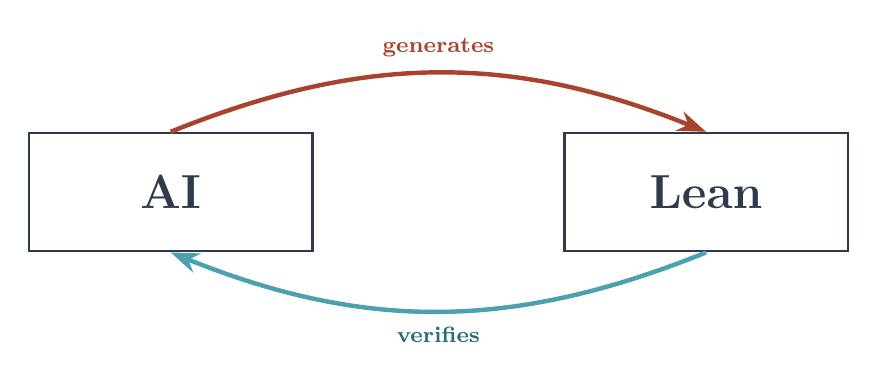
\begin{tikzpicture}[
      node distance=0pt,
      term/.style={rectangle, draw=jtslate, line width=0.9pt, fill=white,
        minimum width=3.6cm, minimum height=1.5cm, align=center,
        font=\fontsize{17}{21}\selectfont\bfseries, text=jtslate},
      flow/.style={-{Stealth[length=3.6mm,width=2.6mm]}, line width=1.6pt},
      lab/.style={font=\bfseries\footnotesize, inner sep=4pt},
    ]

    \node[term] (ai)   at (-3.4,0) {AI};
    \node[term] (lean) at ( 3.4,0) {Lean};

    \draw[flow, jtcopper] (ai.north) to[bend left=22]
      node[lab, above=1pt, midway, text=jtcopperink] {generates} (lean.north);
    \draw[flow, jtteal] (lean.south) to[bend left=22]
      node[lab, below=1pt, midway, text=jttealink] {verifies} (ai.south);

  \end{tikzpicture}
  \end{center}
  \vfill
\end{frame}

%%%%%%%%%%%%%%%%%%%%%%%%%%%%%%%%%%%%%%%%%%%%%%%%%%%%%%%%%%%%%%%%%%%%%%%%%%%%%%%
%  3.9  END OF TECHNICAL INTERLUDE
%%%%%%%%%%%%%%%%%%%%%%%%%%%%%%%%%%%%%%%%%%%%%%%%%%%%%%%%%%%%%%%%%%%%%%%%%%%%%%%
{
\setbeamertemplate{background}{\jtBackgroundDark}
\setbeamertemplate{footline}{}
\begin{frame}[plain]
  \vfill
  {\color{jtondarka}\Large\jtturn}\par
  \vspace{14pt}
  {\color{jtondark}\fontsize{30}{36}\selectfont\bfseries End of technical interlude\par}
  \vfill
\end{frame}
}

%%%%%%%%%%%%%%%%%%%%%%%%%%%%%%%%%%%%%%%%%%%%%%%%%%%%%%%%%%%%%%%%%%%%%%%%%%%%%%%
%  3.10  A LOOK TOWARDS MATHEMATICS
%%%%%%%%%%%%%%%%%%%%%%%%%%%%%%%%%%%%%%%%%%%%%%%%%%%%%%%%%%%%%%%%%%%%%%%%%%%%%%%
\begin{frame}{How good is AI-driven formalisation now?}
  \vfill
  \begin{jtquote}[left=20pt,right=20pt,top=13pt,bottom=13pt]{jttealink}
    {\fontsize{17}{24}\selectfont\color{jtslate}%
      It can essentially formalise {\bfseries anything you want}.\par}
    \vspace{8pt}
    % Details from Anthropic's own write-up, "Formalizing Fermat's Last
    % Theorem in Lean" -- see ../BathSeptember26/FormalizationFermat.png.
    {\fontsize{11}{15}\selectfont\color{jtgrey}%
      Anthropic's Claude formalised
      \href{https://github.com/anthropics/fermats-last-theorem}{%
        \color{jtgrey}Fermat's Last Theorem}
      in Lean in about eleven days, on Lean's three standard axioms alone
      and with no \texttt{sorry}s.\par}
  \end{jtquote}

  \vspace{8pt}
  \onslide<2->{%
  \begin{jtblock}[top=12pt,bottom=12pt]{jtcopper}{}
    {\fontsize{17}{24}\selectfont\color{jtslate}%
      However, this does not necessarily mean
      {\bfseries\color{jtcopperink}well}.\par}
  \end{jtblock}}
  \vfill
\end{frame}

%%%%%%%%%%%%%%%%%%%%%%%%%%%%%%%%%%%%%%%%%%%%%%%%%%%%%%%%%%%%%%%%%%%%%%%%%%%%%%%
%  3.11  FORMALISATION IS NOT COMPLETE TRUST
%%%%%%%%%%%%%%%%%%%%%%%%%%%%%%%%%%%%%%%%%%%%%%%%%%%%%%%%%%%%%%%%%%%%%%%%%%%%%%%
\begin{frame}[fragile]{Formalisation does not give you complete trust}
  \lstset{basicstyle=\ttfamily\scriptsize\color{jtslate}}
  \vfill
  \begin{columns}[T,onlytextwidth]

    \begin{column}{0.40\textwidth}
      \begin{jtquote}[top=12pt,bottom=12pt]{jtcopper}
        {\fontsize{14}{19}\selectfont\color{jtslate}%
          Formalisation is not the whole picture, and should not give you
          the whole trust.\par}
      \end{jtquote}
    \end{column}

    \begin{column}{0.56\textwidth}
      \begin{jtblockcap}[top=5pt,bottom=3pt]{jtcopper}{Fermat's Last Theorem, made trivial}
\begin{lstlisting}
-- "the integers"
def MyInt : Type := Empty

def add (a b : MyInt) : MyInt :=
  Empty.elim a
def pow (a : MyInt) (n : Nat) : MyInt :=
  Empty.elim a

theorem flt (a b c : MyInt)
    (n : Nat) (hn : 3 <= n) :
    Ne (add (pow a n) (pow b n)) (pow c n) :=
  Empty.elim a
\end{lstlisting}
      \end{jtblockcap}
      \vspace{2pt}
      {\fontsize{8}{10}\selectfont\color{jtgrey}%
        Lean accepts it. Nothing here is about numbers.\par}
    \end{column}

  \end{columns}
  \vfill
\end{frame}

%%%%%%%%%%%%%%%%%%%%%%%%%%%%%%%%%%%%%%%%%%%%%%%%%%%%%%%%%%%%%%%%%%%%%%%%%%%%%%%
%  3.12  INGREDIENT 2A OF PHYSICS 2.0  (the Physlib reveal)
%%%%%%%%%%%%%%%%%%%%%%%%%%%%%%%%%%%%%%%%%%%%%%%%%%%%%%%%%%%%%%%%%%%%%%%%%%%%%%%
\begin{frame}{Ingredient 2a of Physics 2.0}
  \vfill
  \begin{jtquote}[top=8pt,bottom=8pt]{jttealink}
    {\fontsize{15}{21}\selectfont\color{jtslate}%
      {\bfseries Physlib} is a {\bfseries corpus of knowledge} whose content
      is {\bfseries formalised into Lean}.\par
      \vspace{4pt}
      Community run, and open source.\par}
  \end{jtquote}

  \vspace{5pt}
  \begin{columns}[T,onlytextwidth]
    \begin{column}{0.475\textwidth}
      \begin{jtblockh}[top=6pt,bottom=6pt]{jttealink}{a dual process}{dual}
        {\fontsize{15}{20}\selectfont\bfseries\color{jtslate}Lean verification\par}
        \vspace{4pt}
        {\jtbody\color{jtgrey}the mathematics\par}
      \end{jtblockh}
    \end{column}
    \begin{column}{0.475\textwidth}
      \begin{jtblockh}[top=6pt,bottom=6pt]{jtcopper}{and}{dual}
        {\fontsize{15}{20}\selectfont\bfseries\color{jtslate}Human review\par}
        \vspace{4pt}
        {\jtbody\color{jtgrey}the physics context, style,
          organisation and quality\par}
      \end{jtblockh}
    \end{column}
  \end{columns}
  \vfill
\end{frame}

%%%%%%%%%%%%%%%%%%%%%%%%%%%%%%%%%%%%%%%%%%%%%%%%%%%%%%%%%%%%%%%%%%%%%%%%%%%%%%%
%  3.13  THE PROBLEM: THE HUMAN HALF
%%%%%%%%%%%%%%%%%%%%%%%%%%%%%%%%%%%%%%%%%%%%%%%%%%%%%%%%%%%%%%%%%%%%%%%%%%%%%%%
\begin{jtproblem}
\begin{frame}{The problem}
  \vfill
  \begin{jtquote}[top=13pt,bottom=13pt]{jtcopper}
    {\fontsize{16}{23}\selectfont\color{jtslate}%
      Lean verification takes the mathematics. But part of the trust still
      rests on {\bfseries human review} --- and that {\bfseries cannot
      scale}.\par}
  \end{jtquote}
  \vfill
\end{frame}
\end{jtproblem}

%%%%%%%%%%%%%%%%%%%%%%%%%%%%%%%%%%%%%%%%%%%%%%%%%%%%%%%%%%%%%%%%%%%%%%%%%%%%%%%
%  3.14  INGREDIENT 2B OF PHYSICS 2.0
%%%%%%%%%%%%%%%%%%%%%%%%%%%%%%%%%%%%%%%%%%%%%%%%%%%%%%%%%%%%%%%%%%%%%%%%%%%%%%%
\begin{frame}{Ingredient 2b of Physics 2.0}
  \vfill
  \begin{jtquote}[top=11pt,bottom=11pt]{jtcopper}
    {\fontsize{15}{21}\selectfont\color{jtslate}%
      There is another solution to scaling trust: {\bfseries one-look
      review}, similar to the arXiv.\par}
  \end{jtquote}

  \vspace{12pt}
  \begin{jtblockcap}[top=8pt,bottom=8pt]{jtcopper}{PhyslibAlpha}
    {\fontsize{15}{21}\selectfont\color{jtslate}%
      This is {\bfseries PhyslibAlpha}, and it allows things to
      {\bfseries scale}.\par}
  \end{jtblockcap}
  \vfill
\end{frame}

%%%%%%%%%%%%%%%%%%%%%%%%%%%%%%%%%%%%%%%%%%%%%%%%%%%%%%%%%%%%%%%%%%%%%%%%%%%%%%%
%  3.15  PROJECT STRUCTURE
%%%%%%%%%%%%%%%%%%%%%%%%%%%%%%%%%%%%%%%%%%%%%%%%%%%%%%%%%%%%%%%%%%%%%%%%%%%%%%%
\begin{frame}{Project structure}
  \vfill
  {\jtmeta\color{jtgrey}\jtlabel{Upstream}\quad
    {\normalfont\bfseries\color{jtslate}Mathlib}\par}
  \vspace{7pt}

  \begin{columns}[T,onlytextwidth]

    \begin{column}{0.315\textwidth}
      \begin{jtblockh}{jttealink}{Core}{struct}
        {\fontsize{14}{18}\selectfont\bfseries\color{jtslate}Physlib\par}
        \vspace{4pt}
        {\jtbody\color{jtslate}Curated to a high standard for long-term
         reuse.\par}
      \end{jtblockh}
    \end{column}

    \begin{column}{0.315\textwidth}
      \begin{jtblockh}{jtcopper}{Rapid}{struct}
        {\fontsize{14}{18}\selectfont\bfseries\color{jtslate}PhyslibAlpha\par}
        \vspace{4pt}
        {\jtbody\color{jtslate}Lighter review, for large-scale AI-assisted
         contributions.\par}
      \end{jtblockh}
    \end{column}

    \begin{column}{0.315\textwidth}
      \begin{jtblockh}{jtgrey}{QI}{struct}
        {\fontsize{14}{18}\selectfont\bfseries\color{jtslate}QuantumInfo\par}
        \vspace{4pt}
        {\jtbody\color{jtslate}Quantum information theory, being brought
         closer to Physlib.\par}
      \end{jtblockh}
    \end{column}

  \end{columns}

  \vspace{7pt}
  {\jtmeta\color{jtgrey}\jtlabel{Adjacent}\quad
    {\normalfont\bfseries\color{jtslate}CSLib}\par}
  \vfill
\end{frame}



%%%%%%%%%%%%%%%%%%%%%%%%%%%%%%%%%%%%%%%%%%%%%%%%%%%%%%%%%%%%%%%%%%%%%%%%%%%%%%%
%  3.16  SIMILAR PROJECTS EXIST
%%%%%%%%%%%%%%%%%%%%%%%%%%%%%%%%%%%%%%%%%%%%%%%%%%%%%%%%%%%%%%%%%%%%%%%%%%%%%%%
\begin{frame}{Physlib is one of three main ones}
  \vfill
  \begin{center}
    \jtrepo{leanprover-community}{mathlib4}
      {https://github.com/leanprover-community/mathlib4}
      {The math library of Lean 4.}
      {\faIcon{star}\;4{,}309 \quad \faIcon{code-branch}\;1{,}768\\[2pt]
       \faIcon{users}\;798 \quad \faIcon{clock}\;2021}%
    \hspace{0.25cm}%
    \jtrepo{leanprover-community}{Physlib}
      {https://github.com/leanprover-community/physlib}
      {Physics, digitalised into Lean. Community-driven.}
      {\faIcon{star}\;786 \quad \faIcon{code-branch}\;205\\[2pt]
       \faIcon{users}\;114 \quad \faIcon{clock}\;2024}%
    \hspace{0.25cm}%
    \jtrepo{leanprover}{CSLib}
      {https://github.com/leanprover/cslib}
      {The computer science library of Lean.}
      {\faIcon{star}\;754 \quad \faIcon{code-branch}\;214\\[2pt]
       \faIcon{users}\;50 \quad \faIcon{clock}\;2025}
  \end{center}
  \vfill
\end{frame}

%%%%%%%%%%%%%%%%%%%%%%%%%%%%%%%%%%%%%%%%%%%%%%%%%%%%%%%%%%%%%%%%%%%%%%%%%%%%%%%
%  3.17  WHAT IS IN IT
%%%%%%%%%%%%%%%%%%%%%%%%%%%%%%%%%%%%%%%%%%%%%%%%%%%%%%%%%%%%%%%%%%%%%%%%%%%%%%%
\begin{frame}{Evidence that this can be done at scale and works}
  \vfill
  {\jtmeta\color{jtgrey}Top-level directories of \texttt{Physlib/},
    by lines of Lean.\par}
  \vspace{7pt}

  {\renewcommand{\arraystretch}{1.18}%
  \begin{columns}[T,onlytextwidth]

    \begin{column}{0.47\textwidth}
      {\color{jttealink}\rule{\linewidth}{1.8pt}}\par\vspace{6pt}
      {\footnotesize\color{jtslate}
      \begin{tabular*}{\linewidth}{@{}l@{\extracolsep{\fill}}r@{}}
        Relativity           & 27{,}545 \\
        QFT                  & 20{,}162 \\
        Particles            & 19{,}104 \\
        SpaceAndTime         & 16{,}069 \\
        Mathematics          & 15{,}795 \\
        QuantumMechanics     & 13{,}057 \\
        ClassicalMechanics   & 11{,}784 \\
        Electromagnetism     &  9{,}442 \\
        StringTheory         &  5{,}285 \\
        Units                &  4{,}076 \\
      \end{tabular*}\par}
    \end{column}

    \begin{column}{0.47\textwidth}
      {\color{jtcopper}\rule{\linewidth}{1.8pt}}\par\vspace{6pt}
      {\footnotesize\color{jtslate}
      \begin{tabular*}{\linewidth}{@{}l@{\extracolsep{\fill}}r@{}}
        StatisticalMechanics &  2{,}449 \\
        ProbabilisticTheory  &  2{,}306 \\
        Cosmology            &  1{,}858 \\
        Meta                 &  1{,}773 \\
        FluidDynamics        &  1{,}361 \\
        CondensedMatter      &  1{,}003 \\
        ClassicalFieldTheory &    554 \\
        Thermodynamics       &    432 \\
        Optics               &     48 \\
        LatticeQFT           &     22 \\
      \end{tabular*}\par}
    \end{column}

  \end{columns}}

  \vspace{9pt}
  {\color{jtrule}\rule{\linewidth}{0.7pt}}\par\vspace{5pt}
  {\jtmeta\color{jtslate}\textbf{154{,}125} lines of Lean across
    \textbf{619} files.\par}
  \vfill
\end{frame}

%%%%%%%%%%%%%%%%%%%%%%%%%%%%%%%%%%%%%%%%%%%%%%%%%%%%%%%%%%%%%%%%%%%%%%%%%%%%%%%
%  3.18  EVIDENCE (THE SPECIMEN): THE HIGGS DEMONSTRATION
%%%%%%%%%%%%%%%%%%%%%%%%%%%%%%%%%%%%%%%%%%%%%%%%%%%%%%%%%%%%%%%%%%%%%%%%%%%%%%%
\begin{frame}{Evidence that this can be done at scale and works}
  \vfill
  {\color{jttealink}\rule{3.2cm}{1.8pt}}\par
  \vspace{16pt}
  {\fontsize{22}{27}\selectfont\bfseries\color{jtslate}
    The Higgs boson, in Lean\par}
  \vspace{18pt}
  {\fontsize{14}{18}\selectfont\href{https://live.lean-lang.org/\#url=https\%3A\%2F\%2Fgithub.com\%2Fjstoobysmith\%2FJTSphyslib\%2Fblob\%2FHiggsExample\%2FPhyslib\%2FParticles\%2FStandardModel\%2FHiggsBoson\%2FExample.lean}{%
    \color{jttealink}live.lean-lang.org}\par}
  \vfill
\end{frame}

%%%%%%%%%%%%%%%%%%%%%%%%%%%%%%%%%%%%%%%%%%%%%%%%%%%%%%%%%%%%%%%%%%%%%%%%%%%%%%%
%  3.19  ADDITIONAL BENEFITS OF HAVING PHYSLIB
%  Closes the trust section: what all of this buys physics.
%%%%%%%%%%%%%%%%%%%%%%%%%%%%%%%%%%%%%%%%%%%%%%%%%%%%%%%%%%%%%%%%%%%%%%%%%%%%%%%
\begin{frame}{Additional benefits of having Physlib}
  \vfill
  \begin{minipage}{0.96\textwidth}
    \raggedright
    \jtnumxs{jttealink}{1}{Allows verification of results, both human and AI.}
    \vspace{4pt}
    \jtnumxs{jttealink}{2}{Allows easy reuse, and improvement.}
    \vspace{4pt}
    \jtnumxs{jttealink}{3}{Allows assumptions to be tracked.}
    \vspace{4pt}
    \jtnumxs{jttealink}{4}{Allows one to easily explore and constrain model spaces.}
    \vspace{4pt}
    \jtnumxs{jttealink}{5}{Prevents bit-rot: one corpus, kept compiling.}
    \vspace{4pt}
    \jtnumxs{jttealink}{6}{Avoids duplicated work, and definitions that are
      incompatible with one another.}
    \vspace{4pt}
    \jtnumxs{jtcopper}{7}{AI speed and efficiency makes this feasible.}
  \end{minipage}
  \vfill
\end{frame}

%%%%%%%%%%%%%%%%%%%%%%%%%%%%%%%%%%%%%%%%%%%%%%%%%%%%%%%%%%%%%%%%%%%%%%%%%%%%%%%
%%  SECTION 4  --  COMMUNITY
%%%%%%%%%%%%%%%%%%%%%%%%%%%%%%%%%%%%%%%%%%%%%%%%%%%%%%%%%%%%%%%%%%%%%%%%%%%%%%%
\begin{jtsection}{4}{Community}{Community}
\end{jtsection}



%%%%%%%%%%%%%%%%%%%%%%%%%%%%%%%%%%%%%%%%%%%%%%%%%%%%%%%%%%%%%%%%%%%%%%%%%%%%%%%
%  4.1  WHAT THE COMMUNITY CURRENTLY DOES
%%%%%%%%%%%%%%%%%%%%%%%%%%%%%%%%%%%%%%%%%%%%%%%%%%%%%%%%%%%%%%%%%%%%%%%%%%%%%%%
\begin{frame}{What the community currently does}
  \vfill
  \begin{minipage}{0.94\textwidth}
    \raggedright
    {\color{jtslate}\fontsize{26}{36}\selectfont\bfseries
      Writes papers.\par Reviews for journals.\par}
  \end{minipage}
  \vfill
\end{frame}

%%%%%%%%%%%%%%%%%%%%%%%%%%%%%%%%%%%%%%%%%%%%%%%%%%%%%%%%%%%%%%%%%%%%%%%%%%%%%%%
%  4.2  WHAT WILL THEY DO IN THIS NEW WORLD
%%%%%%%%%%%%%%%%%%%%%%%%%%%%%%%%%%%%%%%%%%%%%%%%%%%%%%%%%%%%%%%%%%%%%%%%%%%%%%%
\begin{jtproblem}
\begin{frame}{What will they do in this new world?}
  \vfill
  \begin{jtquote}[top=13pt,bottom=13pt]{jtcopper}
    {\fontsize{16}{23}\selectfont\color{jtslate}%
      Writing papers, and reviewing for journals, is exactly the work that
      AI is now {\bfseries capable of}.\par}
  \end{jtquote}
  \vfill
\end{frame}
\end{jtproblem}

%%%%%%%%%%%%%%%%%%%%%%%%%%%%%%%%%%%%%%%%%%%%%%%%%%%%%%%%%%%%%%%%%%%%%%%%%%%%%%%
%  4.3  INGREDIENT 3 OF PHYSICS 2.0
%%%%%%%%%%%%%%%%%%%%%%%%%%%%%%%%%%%%%%%%%%%%%%%%%%%%%%%%%%%%%%%%%%%%%%%%%%%%%%%
\begin{frame}{Ingredient 3 of Physics 2.0}
  \vfill
  {\jtmeta\color{jtgrey}Working on the corpus of knowledge ---
    {\bfseries Physlib}.\par}
  \vspace{10pt}
  \begin{columns}[T,onlytextwidth]
    \begin{column}{0.315\textwidth}
      \jtrole{Review}
      \jtrole{Maintenance}
      \jtrole{Refactoring}
    \end{column}
    \begin{column}{0.315\textwidth}
      \jtrole{Foundational work}
      \jtrole{Formalisation}
      \jtrole{Documentation}
    \end{column}
    \begin{column}{0.315\textwidth}
      \jtrole{Extending}
      \jtrole{Adding experiments}
      \jtrole{Building tools}
    \end{column}
  \end{columns}
  \vfill
\end{frame}



%%%%%%%%%%%%%%%%%%%%%%%%%%%%%%%%%%%%%%%%%%%%%%%%%%%%%%%%%%%%%%%%%%%%%%%%%%%%%%%
%  4.4  PEOPLE ARE ALREADY DOING THIS
%%%%%%%%%%%%%%%%%%%%%%%%%%%%%%%%%%%%%%%%%%%%%%%%%%%%%%%%%%%%%%%%%%%%%%%%%%%%%%%
\begin{frame}{People are already doing this}
  \vfill
  \begin{columns}[T,onlytextwidth]
    \begin{column}{0.295\textwidth}
      \jtfigure{jttealink}{100+}{contributors}
    \end{column}
    \hfill
    \begin{column}{0.295\textwidth}
      \jtfigure{jttealink}{7}{maintainers}
    \end{column}
    \hfill
    \begin{column}{0.295\textwidth}
      {\color{jtslate}\fontsize{15}{20}\selectfont\bfseries
        Always looking\\ for more\par}
    \end{column}
  \end{columns}
  \vfill
\end{frame}

%%%%%%%%%%%%%%%%%%%%%%%%%%%%%%%%%%%%%%%%%%%%%%%%%%%%%%%%%%%%%%%%%%%%%%%%%%%%%%%
%  4.5  BUILT FOR THE COMMUNITY
%%%%%%%%%%%%%%%%%%%%%%%%%%%%%%%%%%%%%%%%%%%%%%%%%%%%%%%%%%%%%%%%%%%%%%%%%%%%%%%
\begin{frame}{Built for the community}
  \vfill
  \begin{columns}[T,onlytextwidth]
    \begin{column}{0.46\textwidth}
      \begin{jtblockh}[top=9pt,bottom=9pt]{jttealink}{we refactor}{principles}
        {\fontsize{15}{21}\selectfont\color{jtslate}%
          When a better approach is found, we take it.\par}
      \end{jtblockh}
    \end{column}
    \hfill
    \begin{column}{0.46\textwidth}
      \begin{jtblockh}[top=9pt,bottom=9pt]{jtcopper}{a choice of starting point}{principles}
        {\fontsize{15}{21}\selectfont\color{jtslate}%
          There is no single correct axiomatisation, so we allow a
          {\bfseries choice of starting point}.\par}
      \end{jtblockh}
    \end{column}
  \end{columns}
  \vfill
\end{frame}

%%%%%%%%%%%%%%%%%%%%%%%%%%%%%%%%%%%%%%%%%%%%%%%%%%%%%%%%%%%%%%%%%%%%%%%%%%%%%%%
%  4.6  DIFFICULTIES IN FORMALISING PHYSICS
%%%%%%%%%%%%%%%%%%%%%%%%%%%%%%%%%%%%%%%%%%%%%%%%%%%%%%%%%%%%%%%%%%%%%%%%%%%%%%%
\begin{frame}{Difficulties in formalising physics}
  \vfill
  \begin{minipage}{0.94\textwidth}
    \raggedright
    \jtnum{jtcopper}{1}{Validation does not come with the guarantees of
      verification.}
    \vspace{10pt}
    \jtnum{jtcopper}{2}{One physical concept, many mathematical descriptions.}
    \vspace{10pt}
    \jtnum{jtcopper}{3}{Physics papers aren't written as definitions and
      theorems.}
    \vspace{10pt}
    \jtnum{jtcopper}{4}{How physical assumptions enter.}
  \end{minipage}
  \vfill
\end{frame}

%%%%%%%%%%%%%%%%%%%%%%%%%%%%%%%%%%%%%%%%%%%%%%%%%%%%%%%%%%%%%%%%%%%%%%%%%%%%%%%
%%  SECTION 5  --  RECOGNITION
%%%%%%%%%%%%%%%%%%%%%%%%%%%%%%%%%%%%%%%%%%%%%%%%%%%%%%%%%%%%%%%%%%%%%%%%%%%%%%%
\begin{jtsection}{5}{Recognition}{Recognition}
\end{jtsection}

%%%%%%%%%%%%%%%%%%%%%%%%%%%%%%%%%%%%%%%%%%%%%%%%%%%%%%%%%%%%%%%%%%%%%%%%%%%%%%%
%  5.1  THE PROBLEM WITH CURRENT RECOGNITION
%%%%%%%%%%%%%%%%%%%%%%%%%%%%%%%%%%%%%%%%%%%%%%%%%%%%%%%%%%%%%%%%%%%%%%%%%%%%%%%
\begin{jtproblem}
\begin{frame}{The problem with current recognition}
  \vfill
  \begin{jtquote}[top=11pt,bottom=11pt]{jtcopper}
    {\fontsize{16}{22}\selectfont\color{jtslate}%
      Recognition is currently based only on {\bfseries publishing papers}
      and {\bfseries citations}.\par}
  \end{jtquote}

  \vspace{12pt}
  \begin{jtblock}[top=9pt,bottom=9pt]{jtcopper}{}
    {\fontsize{15}{21}\selectfont\color{jtslate}%
      In this new world that is a {\bfseries poor proxy} for the work that
      actually matters --- because it is precisely the work we have seen AI
      is {\bfseries very capable of}.\par}
  \end{jtblock}
  \vfill
\end{frame}
\end{jtproblem}

%%%%%%%%%%%%%%%%%%%%%%%%%%%%%%%%%%%%%%%%%%%%%%%%%%%%%%%%%%%%%%%%%%%%%%%%%%%%%%%
%  5.2  WHO GETS THE RECOGNITION
%%%%%%%%%%%%%%%%%%%%%%%%%%%%%%%%%%%%%%%%%%%%%%%%%%%%%%%%%%%%%%%%%%%%%%%%%%%%%%%
\begin{frame}{Who gets the recognition?}
  \vfill
  \begin{jtquote}[top=10pt,bottom=10pt]{jttealink}
    {\fontsize{17}{23}\selectfont\color{jtslate}%
      The library is the {\bfseries foundation of truth}.\par}
  \end{jtquote}

  \vspace{10pt}
  \begin{jtblock}[top=9pt,bottom=9pt]{jttealink}{}
    {\fontsize{15}{21}\selectfont\color{jtslate}%
      A separate, {\bfseries arXiv-like system} records contributions ---
      {\bfseries verified}, and usable on a CV.\par}
      \end{jtblock}
  \vfill
\end{frame}

%%%%%%%%%%%%%%%%%%%%%%%%%%%%%%%%%%%%%%%%%%%%%%%%%%%%%%%%%%%%%%%%%%%%%%%%%%%%%%%
%  5.3  INGREDIENT 4 OF PHYSICS 2.0
%%%%%%%%%%%%%%%%%%%%%%%%%%%%%%%%%%%%%%%%%%%%%%%%%%%%%%%%%%%%%%%%%%%%%%%%%%%%%%%
%  Screenshot is ../Images/ContributionsPhyslib.png -- see scripts note in
%  the repo; re-capture before the talk, the report counts drift.
\begin{frame}{Ingredient 4 of Physics 2.0}
  \vfill
  \centering
  {\fontsize{23}{27}\selectfont\bfseries
    \href{https://contributions.physlib.io}{%
      \color{jttealink}contributions.physlib.io}\par}
  \vspace{7pt}
  \href{https://contributions.physlib.io}{%
    \fcolorbox{jtrule}{white}{%
      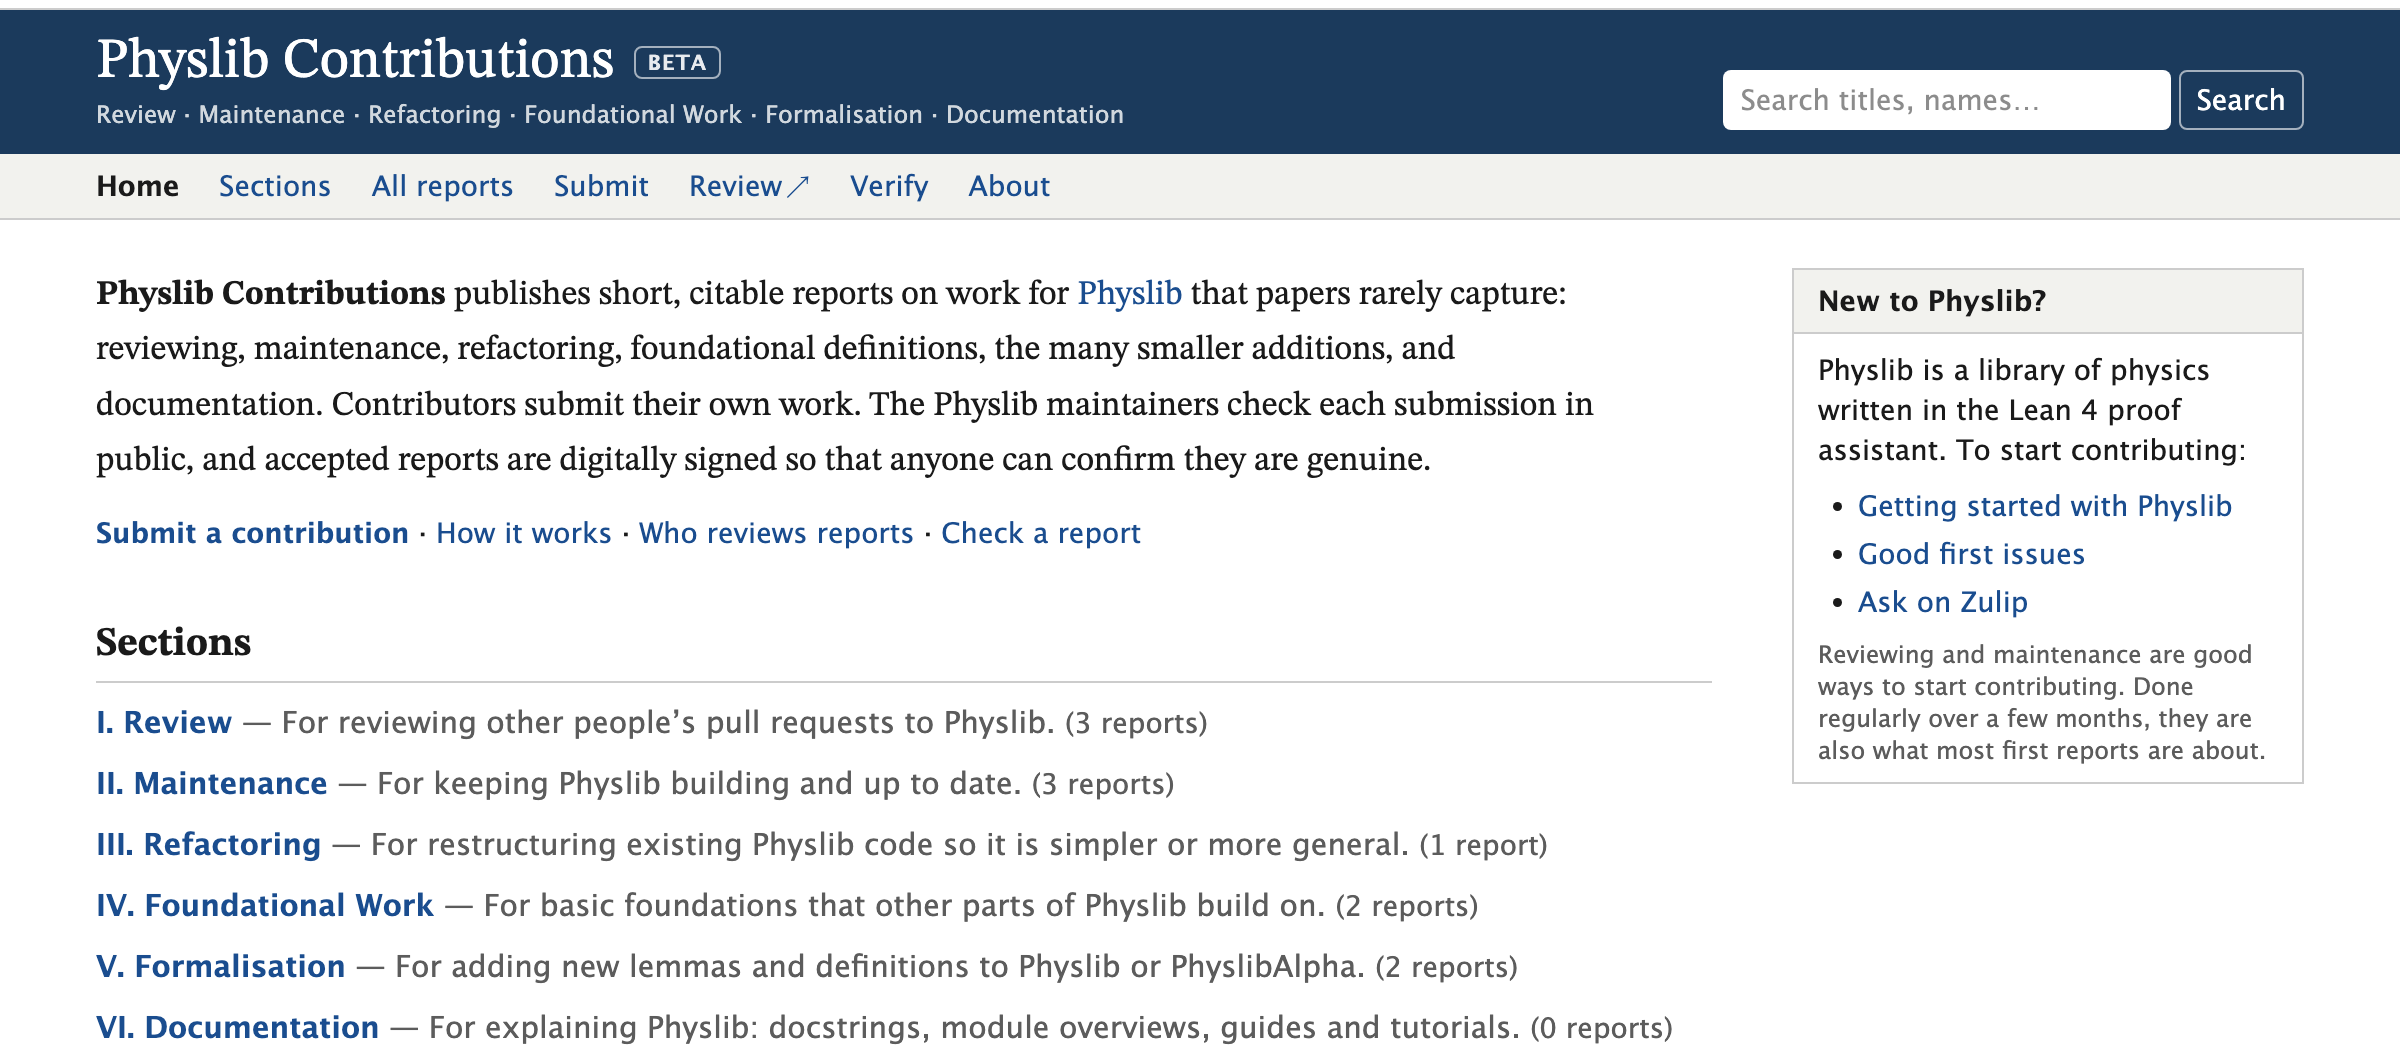
\includegraphics[width=10.5cm]{ContributionsPhyslib.png}}}%
  \par
  \vfill
\end{frame}

%%%%%%%%%%%%%%%%%%%%%%%%%%%%%%%%%%%%%%%%%%%%%%%%%%%%%%%%%%%%%%%%%%%%%%%%%%%%%%%
%%  SECTION 6  --  CONCLUSION
%%%%%%%%%%%%%%%%%%%%%%%%%%%%%%%%%%%%%%%%%%%%%%%%%%%%%%%%%%%%%%%%%%%%%%%%%%%%%%%
\begin{jtsection}{6}{Conclusion}{Conclusion}
\end{jtsection}

%%%%%%%%%%%%%%%%%%%%%%%%%%%%%%%%%%%%%%%%%%%%%%%%%%%%%%%%%%%%%%%%%%%%%%%%%%%%%%%
%  6.1  PHYSICS 2.0  (the headline result; mirrors Physics 1.0)
%%%%%%%%%%%%%%%%%%%%%%%%%%%%%%%%%%%%%%%%%%%%%%%%%%%%%%%%%%%%%%%%%%%%%%%%%%%%%%%
\begin{frame}{Physics 2.0}
  \vfill
  \begin{minipage}{0.96\textwidth}
    \raggedright
  \jtshift{Truth}{Papers}{Physlib}
  \jtshift{Trust}{Peer review}{Lean + human review}
  \jtshift{Community}{Writing papers}{Building and maintaining the corpus}
  \jtshift{Recognition}{Citations}{Contributions recorded and verified}
  \end{minipage}
  \vfill
\end{frame}

%%%%%%%%%%%%%%%%%%%%%%%%%%%%%%%%%%%%%%%%%%%%%%%%%%%%%%%%%%%%%%%%%%%%%%%%%%%%%%%
%  6.2  CALL TO ACTION
%%%%%%%%%%%%%%%%%%%%%%%%%%%%%%%%%%%%%%%%%%%%%%%%%%%%%%%%%%%%%%%%%%%%%%%%%%%%%%%
\begin{frame}{Call to action}
  \vfill
  \begin{columns}[T,onlytextwidth]

    \begin{column}{0.475\textwidth}
      \begin{jtblockh}{jttealink}{If you are hiring, or on grant committees}{cta}
        {\jtbody\color{jtslate}Start to recognise contributions to projects
         like \textbf{Physlib}, \textbf{Mathlib} and \textbf{CSLib} on a
         par with papers.\par}
      \end{jtblockh}
    \end{column}

    \begin{column}{0.475\textwidth}
      \begin{jtblockh}{jtcopper}{If you are an expert in physics}{cta}
        {\jtbody\color{jtslate}Come to \textbf{Physlib}, help review, help
         push forward your area of expertise.\par}
      \end{jtblockh}
    \end{column}

  \end{columns}

  \vspace{16pt}
  % the whole of the passage opened on "What I think"; here it closes the talk
  {\fontsize{13}{18}\selectfont\itshape\color{jtslate}%
    ``Optimism is a duty. The future is open. It is not predetermined. No one
    can predict it, except by chance. We all contribute to determining it by
    what we do. We are all equally responsible for its success.''\par}
  \vspace{2pt}
  {\jtmeta\color{jtgrey}--- Karl Popper, \emph{The Lesson of This Century}\par}
  \vfill
\end{frame}

%%%%%%%%%%%%%%%%%%%%%%%%%%%%%%%%%%%%%%%%%%%%%%%%%%%%%%%%%%%%%%%%%%%%%%%%%%%%%%%
%  6.3  THANK YOU
%%%%%%%%%%%%%%%%%%%%%%%%%%%%%%%%%%%%%%%%%%%%%%%%%%%%%%%%%%%%%%%%%%%%%%%%%%%%%%%
{
\setbeamertemplate{background}{\jtBackgroundDark}
\setbeamertemplate{footline}{}
\begin{frame}[plain]
  \vfill
  \begin{columns}[T,onlytextwidth]
    \begin{column}{0.97\textwidth}
      {\color{jtondarka}\rule{3.2cm}{2pt}}\par
      \vspace{18pt}

      {\color{jtondark}\fontsize{30}{35}\selectfont\bfseries
        Thank you for watching\par}

      \vspace{24pt}
      {\color{jtondarkm}\rule{\linewidth}{0.5pt}}\par
      \vspace{12pt}

      {\color{jtondark}\fontsize{13}{16}\selectfont\bfseries Joseph Tooby-Smith\par}
      \vspace{4pt}
      {\color{jtondarkm}\jtmeta University of Bath\par}

      \vspace{14pt}
      {\color{jtondarkm}\jtmeta
        \href{https://github.com/leanprover-community/physlib}{%
          \color{jtondarkm}github.com/leanprover-community/physlib}
        \qquad
        \href{https://contributions.physlib.io}{%
          \color{jtondarkm}contributions.physlib.io}
        \qquad
        \href{https://josephtoobysmith.com/}{%
          \color{jtondarkm}josephtoobysmith.com}\par}
    \end{column}
  \end{columns}
  \vfill
\end{frame}
}

\end{document}
